\documentclass{article}


% Packages
\usepackage[utf8]{inputenc} % For Norwegian letters
\usepackage{tabulary} % For nice tables
\usepackage{parskip} % For vertical spacing between paragraphs
\usepackage{float}
\usepackage{graphicx}
\usepackage{caption}
\usepackage{subcaption}
\usepackage{listings}
\usepackage{enumitem}
\usepackage[obeyspaces]{url}

% Config
\setlength{\parindent}{0cm}
\setlength{\parskip}{\baselineskip}

\graphicspath{{images/}}

\begin{document}

% Title
\title{\textbf{Exercise 4} \\ TDT4173}
\author{Simon Borøy-Johnsen \\ MTDT}
\date{\today}
\maketitle
% End Title


% Content
\section{Theory}
\subsection*{Bayesian Learning}
\begin{enumerate}
    \item
        The notion of likelihood is used to quantify how likely the occurrence of an event is. One can for example describe the likeliness of observing some data given the source of that data.
    
        $h_{MAP}$ describes the hypothesis that is most likely to occur, given the likelihood of the hypothesis itself, in addition to observed data. $h_{ML}$ assumes all hypotheses are equally likely, and describes the hypothesis that is most likely given the observed data.
    
        A hypothesis can be $h_{MAP}$ without being $h_{ML}$. This happens when we know something about the likelihood of the initial hypothesis.
    
        An example of a hypothesis that is $h_{MAP}$ without being $h_{ML}$ can be showed when classifying spam mail. Using a $h_{ML}$, we will assume that it is the same probability that a random mail is spam as the probability of it being relevant. With $h_{MAP}$, we know that there is a lot more spam that relevant mail, and incorporate this into the classifying system.
    
    \item
        When building an Optimal Bayes classifier, one have to calculate the probabilities of all the hypotheses (given the data), and then the probabilities for all classifications given the hypotheses.

        When building a Naive Bayes classifier, one have to go through every target value, estimating its probability. Then, for each attribute, calculate the probability of the attribute given the target value.
        
        The Brute Force Map can be used, as this tries to calculate the probabilities of the hypotheses, just like the Optimal Bayes classifier.
        
        A Naive Bayes classifier is an approximation of an Optimal Bayes classifier, assuming the features are conditionally independent given the class.
        
    \item
        \begin{enumerate}[label=(\alph*)]
            \item A Naive Bayes classifier does not search through any of the hypothesis space, whilst Optimal Bayes searches through the whole hypothesis space.
            
            \item An Optimal Bayes classifier has the best performance, as Naive Bayes is only an approximation. Nevertheless, Naive Bayes still does quite well.
            
            \item An Optimal Bayes classifier iterates over the whole hypothesis space, which usually is far too large to iterate over. A Naive Bayes classifier only store $(|a| + 1) * |v|$ probabilities, where $a$ is the set of all attributes, and $v$ is the set of all classes. A Naive Bayes classifier will also iterate over every attribute for each class, performing the probability multiplications.
        \end{enumerate}
        
    \item
        An Optimal Bayes classifier algorithm will be hard to improve, but decreasing the hypothesis space will increase the computational cost significantly.
        
        A Naive Bayes classifier algorithm is pretty fast already, but adding more relevant attributes will help increase the performance.
        
    \item
        Both Naive Bayes classifiers and Bayesian belief networks use given probabilities to calculate the final probabilities. Whilst a Naive Bayes classifier assumes all attributes are conditionally independent of each other given their classifications (which they rarely are), a Bayesian belief network allows creating joint probability tables for independent attributes, as well as defining more precise tables for dependent attributes.
\end{enumerate}


\section{Practical}
\subsection*{Expectation Maximization}
\begin{enumerate}
    \item
        See main.py.
    
    \item
        \begin{enumerate}[label=(\alph*)]
            \item
                Initial parameters: [-0.60049099999999989, 3.012454].
                
                These parameters were obtained by sorting the initial array, splitting it at the middle, and then calculating the averages for each half.
                
                By doing this, I ensured that the averages were far apart, increasing the probability of the initial parameters coming close to the final results.
            
            \item
                The initial parameters came very close to the final values. After the fifth iteration, the five first digits were already correct. At the thirtieth iteration, the algorithm had converged.
            
                \begin{tabular}{|l|l|l|}
                    \hline
                    \textbf{Iteration} & \textbf{$\mu_1$} & \textbf{$\mu_2$} \\\hline
                    Initial & -0.60049099999999989 & 3.012454 \\\hline
                    5     & -0.5766510525560046 & 2.978387537663326 \\\hline
                    10    & -0.5766685021527731 &  2.9783703125254943 \\\hline
                    Final & -0.5766685631380497 &  2.9783702523488067 \\\hline
                \end{tabular}
                
            \item
                Visualisation:
            
                \begin{figure}[H]
                    \centering
                    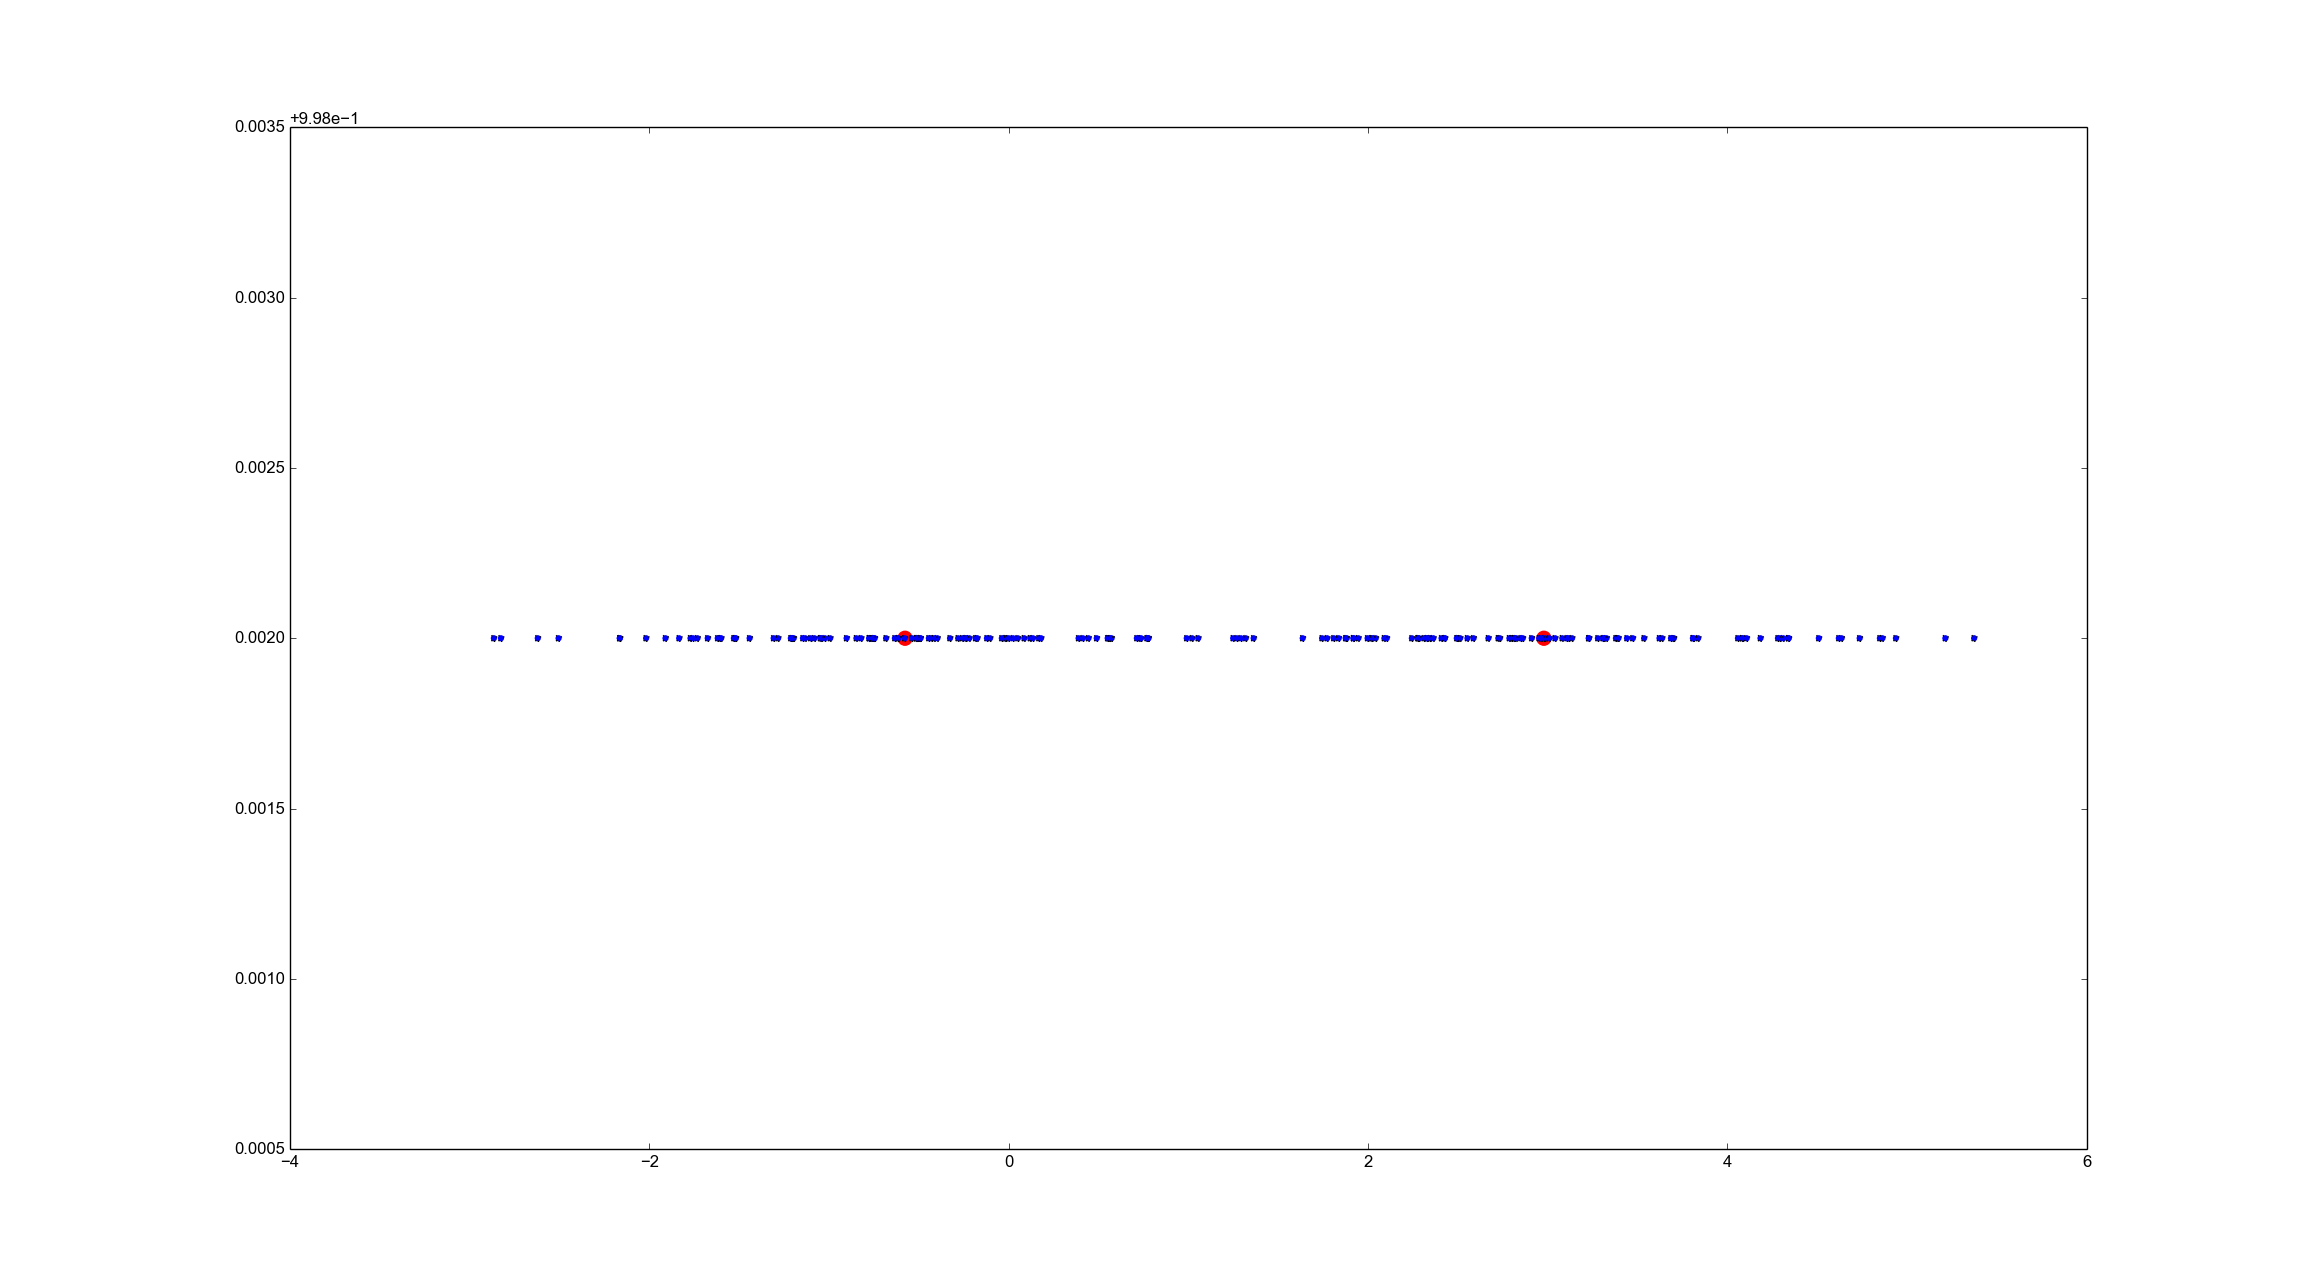
\includegraphics[width=1.0\textwidth]{plot.png}
                    \caption{Plot of the initial data  (blue) and final results (red).}
                \end{figure}
        \end{enumerate}
\end{enumerate}

% End content

\end{document}